\documentclass{article}

% For figures
\usepackage{graphicx} % more modern
\usepackage{subfigure} 
\usepackage{amsfonts}

% For equations
\usepackage{amsmath}

% For citations
% \usepackage{natbib}

\usepackage{booktabs}

% For algorithms
\usepackage{algorithm}
\usepackage{algorithmic}

\usepackage{hyperref}

% Packages hyperref and algorithmic misbehave sometimes.  We can fix
% this with the following command.
\newcommand{\theHalgorithm}{\arabic{algorithm}}

% \usepackage{sty/icml2013} 
% Employ this version of the ``usepackage'' statement after the paper has
% been accepted, when creating the final version.  This will set the
% note in the first column to ``Proceedings of the...''
\usepackage[accepted]{sty/icml2013}


% The \icmltitle you define below is probably too long as a header.
% Therefore, a short form for the running title is supplied here:
\icmltitlerunning{Clustering and Topic Discovery in Gene Expression Data}

\begin{document} 

\twocolumn[
\icmltitle{Bayesian Clustering and Topic Discovery: \\ 
           Adventures with Gene Expression Data}

% It is OKAY to include author information, even for blind
% submissions: the style file will automatically remove it for you
% unless you've provided the [accepted] option to the icml2013
% package.
\icmlauthor{Karren Dai Yang, Skanda Koppula}{\{karren, skoppula\}@mit.edu}
\icmladdress{Massachusetts Institute of Technology,
            Cambridge, MA 02139 USA}

\icmlkeywords{topic models, bayesian clustering, gene expression, gene modules}

\vskip 0.3in
]

\section{Introduction}
\label{intro}
Tumors cell lines are composed of different sub-populations of cells which often exhibit shared patterns of gene expression. Biologists are interested in two key questions: given gene expressions values, (1) can we identify biologically meaningful gene modules, and (2) can we identify cell sub-populations and find gene modules that illuminate their differences? Our goal with this project was to address these questions using Bayesian methods.

To address the first question, we explored the use of Latent Dirichlet Allocation (LDA), two non-parametric topic models, and a dynamic-topic LDA. To address the second question, we explored the use of a finite mixture model as well as a clustering topic model.

\subsection{Description of Data}
To do our analysis, we used a single-cell RNA-sequencing (scRNA-seq) dataset obtained from human melanoma samples \cite{melanoma}. The data consisted of the expression values of 22,712 genes for each of 4645 cells. In total, the dataset amounted to 0.86 GB, presenting significant computational challenges when attempting posterior inference. Apart from a few computational tricks (online inference, multi-core parallelization), for most methods, we pruned non-informative genes from the dataset, ranking based on the deviation in value across cells \footnote{We recognize that this can bias towards noisy genes. We favor this method because it is simple and easy to implement, and a practice used in literature \cite{pruning}}. The Seurat biological toolkit in R was also used for the purpose of low-variance feature selection \cite{seurat}. We eschewed dimensionality reduction techniques such as PCA because of loss of its direct feature interpretability. Prior researchers have labeled the cells in our dataset; there are a total of 9 cell categories \cite{melanoma}. The complete dataset, as well our preprocessed and pruned versions, are openly available \cite{dataset}.

\subsection{Prior work}
Prior research has explored the use of various computational techniques to analyze gene expression data. Most commonly, Spearman and Pearson correlation metrics are frequently used infer sets of genes that cluster together \cite{profiling, nature}. Other techniques, including PCA followed by linear regression, has been used for expression-based cell clustering \cite{transcriptomics}. Yu et al. propose an unsupervised classifier ensemble as another approach to cell clustering \cite{consensus}. 

More Bayesian approaches have also been tried in prior work from the Pe'er lab. \cite{bayesge2} uses a Heirarchical Dirichlet Mixture Model to learn cell clusterings. \cite{bayesge1} builds on this to jointly learn optimal normalization pre-processing of the data. Bayesian networks have also been used in an attempt to learn gene dependencies from expression data \cite{bayesge3}. Our work uses different models to explore gene expression data, but where appropriate (e.g. LDA vs. non-parametric models), we compare results.

\subsection{Structure of Report}
We first discuss our experiments using Bayesian topic models to discover topics in scRNA-seq data: LDA in Section~\ref{ldasec}, non-parametric topic models in Section ~\ref{nonparametricsec} and Dynamic Time Models in Section~\ref{dtmsec}. Then, we discuss our experiments in clustering: Finite Mixtures in Section~\ref{mmsec}, and Integrated Topic-Clustering in Section~\ref{intsec}. We conclude our paper with our observations from across all our studies.

For the purpose of reproducibility, all code can be found at \url{https://github.com/skoppula/882}.

\section{Latent Dirichlet Allocation} 
\label{ldasec}
\subsection{Model Description} 
In the generative process for LDA, the topic assigned to each word is a drawn from the document's topic distribution. The identity of the word is drawn from topic's word distribution. Assuming the reader is familiar with LDA, we relegate further details and formalization of the model to \cite{LDA}.

In the context of analyzing gene expression data, we are interested in discovering 'topics' that comprise of a set of top-$N$ genes within the topic distribution that are biologically related. For example, together the genes may direct a specific chemical function in a cell. Biologists denote such sets of genes as 'gene modules' which can be cross-referenced with existing gene module databases.

\subsection{Implementation} 
A first attempt using the built-in Python \texttt{lda} package resulting in early memory overflows during what we suspect was pre-allocation of per-document variables. The source code was not available, so we had few clues.

We switched to two open-source implementations: an online mean-field variational Bayes for posterior estimation \cite{ovb}, and a broken \texttt{C++} Gibbs sampler for LDA \cite{plda}. 

\nocite{online}

We fixed portions of the sampler to compile properly and extended the sampler to run across four cores. Details of our sampling procedure can be found in Appendix~\ref{ldaappendix}. We compared these two posterior estimation approaches using our entire dataset, using a 10\% held-out testing partition. We experimented using $k=5, 10, 25, 50$ topics. We did not require dataset pruning after these optimizations.

\subsection{Experiments} 
We evaluated the interpretability of our topics (ranked lists of genes) using hypergeometric tests \cite{hg}. In brief, this determines the enrichment of our topics for any existing collections of genes catalogued by biologists in the gene module database \texttt{MSigDB} \cite{msigdb}. More details about the score can be found in the Appendix.

Figure~\ref{fig:pathways} in the Appendix shows gene module matches in \texttt{MSigDB} for which the $p$-value of the match is at least less than 0.3. Notice that models with more topics tended to have more matches with higher significance. The $p$-values in our tests do \textit{not} factor for multiple hypothesis corrections, so at the moment we are only using them as relative measures of model quality.

It is validating to see that many of the similar modules, such as the \texttt{BRCA1} and \texttt{DOXORUBICIN}, are cancer related, given that our expression assay was from tumor cells.

Extracting the parameters of each model, we calculated log-likelihood on our held-out test set. This is shown in Figure \ref{fig:ll}. We found that for this dataset increasing the topic count increases log-likelihood, roughly linear from 5 to 50. Further experiments will need to test at what point log-likelihood drops off; this is one way to optimize the number of topics.

\begin{figure}
    \centering
    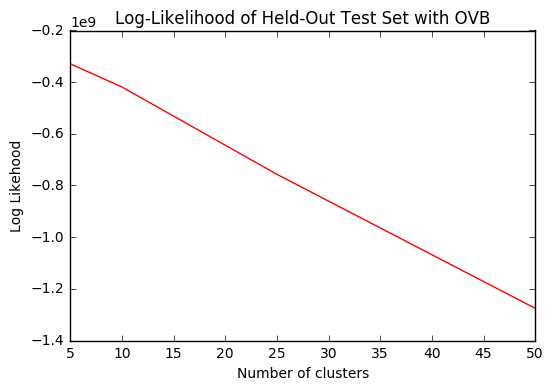
\includegraphics[width=0.4\textwidth]{figs/ll}
    \caption{Log-likelihood of the held-out testing set across numbers of topics. Higher topic sizes are explored in later models.}
    \label{fig:ll}
\vskip -0.2in
\end{figure}


As an interesting aside, Figure \ref{fig:time} shows the time until inference completion (collected during our experiments). Gibbs appears to scale poorly with the parameter dimensionality, in contrast to online variational Bayes \footnote{It is important to note that comparing the magnitude of the time to complete inference in Figure~\ref{fig:time} is not particularly meaningful; as described in Appendix~\ref{ldaappendix}, we chose a reasonable guess for the number of iterations
and optimization threshold after which to stop estimation}. 

\begin{figure}
    \centering
    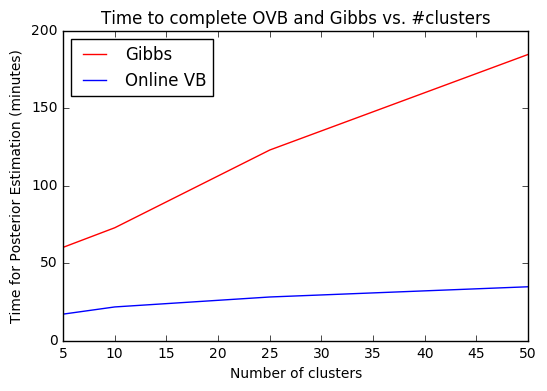
\includegraphics[width=0.4\textwidth]{figs/time}
    \caption{Comparison of the running times of each of the posterior estimation methods across various numbers of topics. Termination conditions across all runs were constant, and described in Appendix~\ref{ldaappendix}}
    \label{fig:time}
\end{figure}

Posterior predictive checks to test the mutual information between the each cell and its words' topics is something that we did not have time, but would be interesting to examine. It's not clear that this independence assumption is true in the context of gene expression data, because of cross-talk and regulatory mechanisms between gene modules.

\section{Non-Parametric Topic Models} 
\label{nonparametricsec}
\subsection{Model Description}
One limitation of LDA is the need to define the number of topics a priori. Non-parametric models overcome this limitation by assuming a countably infinite number of topics. We trained and compared two non-parametric topic models with LDA: the Hierarchical Dirichlet Process (HDP) and the Indian Buffet Process Compound Dirichlet Process (IDP-DP). On a high level, HDP is very similar to LDA, with the main difference being that the draws from a Dirichlet distribution in LDA are replaced with draws from a Dirichlet process in HDP \cite{HDP}. One drawback to the HDP is that there tends to be a correlation between how frequently a topic appears across all documents and how prevalent this topic is within documents that it appears in. This may be undesirable in circumstances where there are 'rare' topics with high prevalence in a small number of documents. IBP-DP tries to overcome this problem by separately modeling the frequency of documents that contain a topic and the prevalence of this topic within a document where it is present \cite{HDP}. Both generative models are described in greater detail in the Appendix (sections \ref{HDP-details} and \ref{IBP-details}).

\subsection{Experiment: LDA vs. HDP}

We trained an HDP topic model and compared it to LDA models with similar numbers of topics, using held-out perplexity and gene set enrichment analysis as described above as our evaluation metrics. We used an existing C++ implementation of the Gibbs sampler provided by the authors of the original paper \cite{HDP}. Since the available implementation of the posterior inference algorithm for HDP was too slow to run on the entire dataset, we did feature selection using the Seurat toolkit in R \cite{seurat} to reduce the number of genes in our dataset with low variance across cells, and trained all models on this subset of data. We tuned the concentration parameters in HDP to obtain a reasonable number of topics (i.e. ~150); subsequently, we trained LDA models with similar numbers of topics for comparison. We found that the HDP model had higher perplexity on a held-out dataset (Figure \ref{fig:hdp-perplexity}). Moreover, the topics in the HDP model tended to have less significant enrichment for known gene sets from \texttt{MSigDB}, and we found that this difference to be significant (Figure \ref{fig:hdp-enrichment}, Mann-Whitney-U test, $p<0.0001$). Overall, the LDA model proved superior to the HDP model in this experiment.

\subsection{Experiment: LDA vs. IBP-DP}
One drawback to the HDP is that there tends to be a correlation between how frequently a topic appears across all documents and how prevalent this topic is within documents that it appears in. Williamson et al. \cite{IBP} proposed the 'focused topic model' to overcome this drawback. We implemented their model to compare it with LDA on the Reuters-21578 dataset. Since the code from the original IBP-DP paper was not available, we implemented an inference algorithm using collapsed Gibbs sampling \cite{IBP}. Due to the non-conjugacy of the model, sampling each latent variable from its full conditional required using another sampling method. To sample the topics parameters, the number of which changes depending on how many topics are represented in the dataset, we used slice sampling based on the semi-ordered stick-breaking representation of the model \cite{IBP2}. For more details about implementation, please refer to those papers.\\

We tested our code on a subset of the Reuters-21578 dataset, using several different values of the concentration hyper-parameter $\alpha$, which influences the number of clusters. Although higher values of $\alpha$ yielded better log-likelihood values, we found that it resulted in a large number of very small topics, which are not very useful (Figure \ref{fig:ibp_words_in_topic}). Qualitatively, we did not find the topics from IBP-DP (Figure \ref{fig:ibptopics}) to be more coherent than topics than LDA (Figure \ref{fig:ldatopics}). The most prevalent topics from the IBP-DP each corresponded to similar topics from LDA; less prevalent topics tended to consist of a few unrelated words. These results discouraged us from optimizing the code to train this model on our scRNA-seq dataset, as we do not think it would yield more coherent gene modules than LDA. We emphasize that these results are not completely unexpected, as the authors of the IBP-DP paper did not show any topics from their model, nor did they assess the quality of their model with metrics other than perplexity.

\section{Dynamic Topic Model} 
\label{dtmsec}
\subsection{Model Description} 
As tumor cells proliferate, they undergo a process called \textit{differentiation}. The set of cells types during tumor emergence may differ from the set of types expressed days later. Correspondingly, patterns of gene expression may also change over time. The set of gene modules expressed in the cells, or the composition of each gene module (topic), may also change.

To capture these evolving topics, we look to dynamic topic models \cite{dtm}. In brief, dynamic topic models establish a conditional distribution over the hyperparameters $\alpha$ and $\beta$, that govern the document's topic distribution and topic's word distribution, respectively. The distribution over each hyperparameter is conditioned on the prior in the previous time step, allowing changes to topic composition and assignment. This can be seen graphically in the plate
model in Figure~\ref{fig:dtmplate}. For convenience, we provide a concise description of the generative process for the implemented heirarchical model for a time slice $t$ in Appendix~\ref{dtmappendix}.

\begin{figure}[h]
    \vspace{-0.1in}
    \centering
    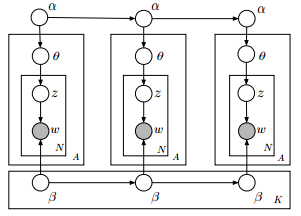
\includegraphics[width=0.4\textwidth]{figs/dtmplate}
    \caption{Plate diagram for the Dynamic Topic Model. Reproduced from \cite{dtm}.}
    \label{fig:dtmplate}
    \vspace{-0.1in}
\end{figure}

Note that in contrast to LDA, dynamic topic models use a logistic-normal to express proportion uncertainty. This is stated more explicitly in Appendix~\ref{dtmappendix}.

\subsection{Implementation}

Unfortunately, due to the non-conjugacy of the Gaussian/Multinomial in our logistic-normal setup, integrating out parameters for any sort of Gibbs sampling becomes hard. Instead, the original DTM paper uses a variational approximation based on a Kalman filter, that preserves time dependencies, unlike a mean-field approximation.

Re-implementing the variational approximation, while educational and interesting, would be a project of itself, so our first attempt in employing dynamic time models to our gene expression data re-used the Kalman Filter-based variational inference used by the original authors, published recently by the Blei Lab \cite{dtmbleigit}. The results we show in the subsequent section are using a wrapper we've implemented around the group's inference code.

The authors stumbled upon a recent arXiv pre-print that proposed a set of sampler update rules to create a correct DTM Gibbs sampler \cite{sdtm}. Using the probabalistic programming framework \texttt{Edward}, and modifying the in-built sampler to follow these updates, we were able to obtain a working Gibbs-sampler for sample time-sliced data for a dynamic topic model defined in Edward \cite{edward}. While we don't have time to conduct benchmarks or re-run our results right now, after verifying that results are consistent, the authors hope to submit a merge for this Edward sketch into the mainstream Edward examples library this coming summer.

\subsection{Experiments} 
We subdivided our data into three seperate time slices, and pruned each slice, retaining the top 20\% of high-variance genes. We experimented using $k=15$, $30$, and $50$ topics.

Similar to our analysis in Section~\ref{ldasec}, we used the hypergeometric test to evaluate interpretability. 

Figure~\ref{fig:pathwaysdtm} in the Appendix shows gene module matches for which the $p$-value is less than 0.3, across the three time slices and the three topic count sizes. Interestingly, we notice a very different set of matched gene modules, with exception of the \texttt{KLF1} module\footnote{This could very well be a result of our dataset pruning, which we did to keep inference runtimes manageable}. Like before, we notice that some of the identified topics are relevant to tumor cells:
\texttt{ST\_TUMOR\_NECROSIS\_FACTOR\_PATHWAY} and \texttt{WEST\_ADRENOCORTICAL\_TUMOR\_MARKERS\_UP} to name the two most prominent topics.

We do not see that much variation across time-slices, demonstrating that our time-slice partitions are largely uniform. For example, for model $k=50$, we see that topic 20 consistently matches with MSigDB module \texttt{PILON\_KLF1\_TARGETS\_UP}, suggesting that its gene composition is not varying.

Models with more topics tended to have more matches with higher significance. But again, the $p$-values in our tests do \textit{not} factor for multiple hypothesis corrections, so at the moment we are only using them as relative measures of model quality.

After extracting the mode of learned parameters, we evaluated the log-likelihood of our held-out test set, also partitioned by time. This is shown in Figure \ref{fig:lldtm}. We find a leveling of log-likelihood after $k=30$.

\begin{figure}
    \centering
    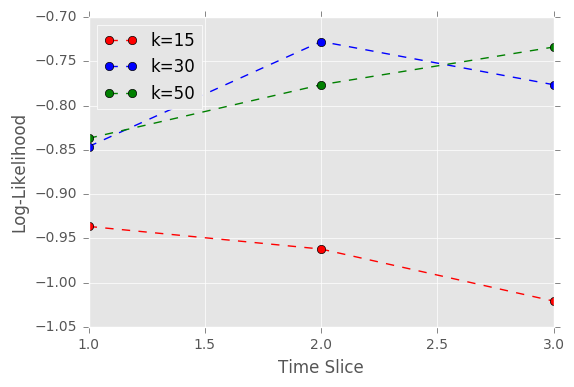
\includegraphics[width=0.4\textwidth]{figs/lldtm}
    \caption{Log-likelihood of the held-out testing set across our time slices for varying numbers of topics.}
    \label{fig:lldtm}
\vskip -0.2in
\end{figure}

With more time, we would ideally repeat the experiments to obtain confidence intervals on these experiments, and examine the gene-module/cell/time-slice mutual information.

\section{Mixture Model} 
\label{mmsec}
\subsection{Model Description} 
The second question -- whether we could learn cell groupings -- we tackled using a canonical Gaussian mixture model. In brief, the model assigns every data point to a cluster; every cluster is Gaussian whose parameters are learned through posterior inference. A plate diagram can be found at \cite{mmplate}. This model is different from the previously mentioned Pe'er papers which use Dirichlet Processes Mixtures to study expression data. By plotting 
histograms of whitened gene expression values, we've found that for many genes the distribution is Gaussian across our data points. This hints that the generative process in a Gaussian mixture model is plausible.

\subsection{Implementation} 
We implemented the mixture model in \textbf{Edward}, the probabalistic programming framework on top of Tensorflow. This allowed us to experiment with different samplers and variational inference approximations. The results we show below are for our runs using a Gibbs sampler, with a fixed burn-in of number of samples (200), a fixed number of sampling iterations (500).

\subsection{Experiments}  
% As a pre-processing step, we normalized every gene to zero-mean, unit variance across the data points. To speed up inference, we cut the dimensionality of the data to 10 using PCA before feeding it into our mixture model.

Figure~\ref{fig:mmplot} shows an estimated cluster assignment for one-hundred sampled data point. We see that while our learned assignments do capture some of the clustering, there is significant bias toward one group (the burgundy cluster).

Following this trend, we examined the set of unique clusters assigned in the posterior. The results are shown in Table~\ref{mmtable}. Interestingly, the model consistently uses less clusters than is allocated in the model. We are unsure why this is the case.

Finally, we examine the log-likelihood of a held-out test set three different runs of posterior estimation with our sampler. This is shown in Figure~\ref{fig:llmm}. The runs are consistent with each other, and the likelihood is largely invariant across the five different cluster counts we tried, $k=\{10,25,50,75,50\}$. There are an estimated 9 true cell types in the original dataset, which could explain this result.

\begin{figure}[h]
    \centering
    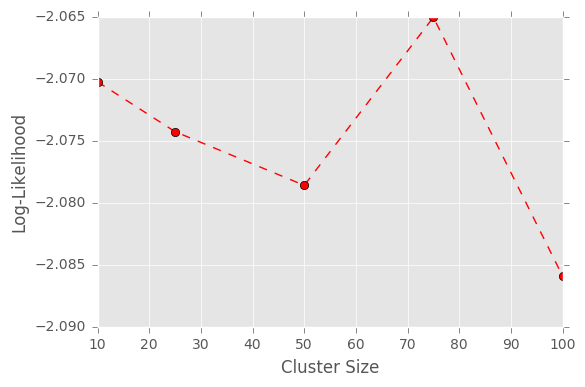
\includegraphics[width=0.4\textwidth]{figs/llmm}
    \caption{Log-likelihood of held-out test set, on three seperate runs of Gibbs sampling procedure, described above}
    \label{fig:llmm}
\end{figure}

\begin{table}[h]
    \centering
    \label{mmtable}
    \begin{tabular}{@{}ll@{}}
        \toprule
        \# of Clusters & \# of Clusters Used \\ \midrule
        10                 & 3                                                         \\
        25                 & 9                                                         \\
        50                 & 16                                                        \\
        75                 & 18                                                        \\
        100                & 20                                                        \\ \bottomrule
    \end{tabular}
    \caption{The number of clusters defined in the model appears to be more than the actual number of unique clusters assigned to the data points after posterior estimation. The estimated true number of categories is 9.}
\end{table}


\begin{figure*}[ht]
    \centering
    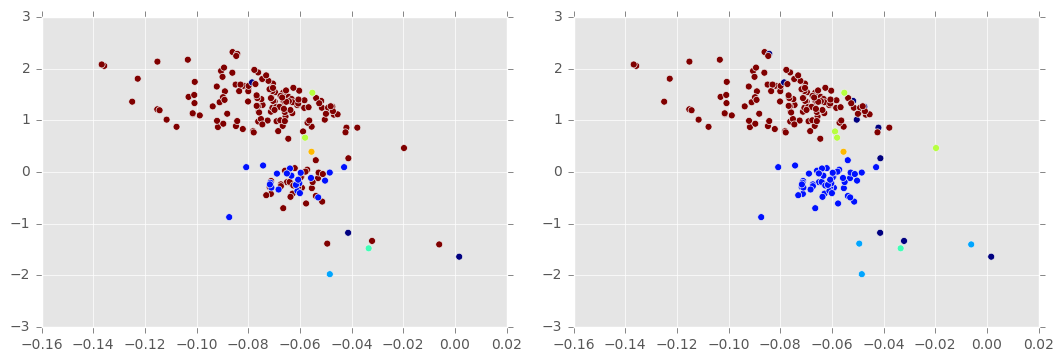
\includegraphics[width=0.9\textwidth]{figs/totalclusters}
    \caption{2D-projection of sampled gene expression data points, colored by predicted cluster (left) and by true cluster assignments (right). Axis are the two learned PCA dimensions.}
    \label{fig:mmplot}
\vskip -0.2in
\end{figure*} 


\section{Integrated Topic-Clustering Model} 
\label{intsec}
\subsection{Model Description}
LDA is suitable for modeling corpuses with no special structure, but this is not the case of scRNA-seq data. Since the cells within a tissue sample may belong to many different sub-populations, we would expect cells within the same sub-population to have more similar topic proportions. We capture this additional structure using the clustering topic model (CTM), a unified framework for clustering and topic modeling based on LDA. In this model, which is similar to the one proposed by \cite{wallach_thesis}, the following generative process is assumed:

\begin{enumerate}
\item Choose a distribution over the clusters, $\pi \sim$ Dir($\pi_0/C$), where $\pi_0$ is a hyperparameter and $C$ is the number of clusters.
\item Choose a global distribution over the topics, $\phi_0 \sim$ Dir($\alpha_0/T$), where $\alpha_0$ is a hyperparameter and $T$ is the number of topics.
\item For each cluster $c$, choose a cluster distribution over the topics, $\phi_c \sim$ Dir($\alpha_1 \phi_0$), where $\alpha_1$ is a hyperparameter
\item For each topic $k$, choose a distribution over the vocabulary, $\beta_k \sim$ Dir($\eta$), where $\eta$ is a hyperparameter.
\item For each document $d$,
\begin{enumerate}
\item Choose a cluster assignment $\xi_d \sim$ Cat($\pi$)
\item Choose a distribution over topics based on the cluster assignment, $\theta_d \sim$ Dir($\alpha \phi_{xi_d}$), where $\alpha$ is a hyperparameter.
\item Choose the number of words in this document, $N_d \sim$ Poisson($\kappa$), where $\kappa$ is a hyperparameter.
\item For the $i$th word in the $d$th document,
\begin{enumerate}
\item Choose a topic, $z_{di} \sim$ Categorical($\theta_d$), based on the distribution over topics
\item Choose a word, $w_{di} \sim$ Categorical($\beta_{z_{di}}$), based on the distribution over the vocabulary for topic $z_{di}$
\end{enumerate}
\end{enumerate}
\end{enumerate}

This model is very similar to LDA, with the addition of cluster assignments that influence document topic proportions. Note that the documents in each cluster have more similar topic proportions, particularly if we choose a reasonably large value of $\alpha$.

\subsection{Inference}
We implemented a collapsed Gibbs sampling in \texttt{MATLAB} to perform inference for the CTM, integrating out all latent variables except the topic assignments $z$ and the cluster assignments $\xi$ to facilitate mixing. First, we establish the prior distribution of $z_{di}$:
\begin{equation} \label{eq:z_prior}
p(z_{di} = k | z_{-di}, \xi_d) = \frac{N_{d,k} + \alpha\frac{N_{\xi_d,k} + \alpha_1\frac{N_k + \alpha_0/K}{N + \alpha_0}}{N_{\xi_d}} + \alpha_1}{N_d + \alpha}
\end{equation}
where $z_{-di}$ refers to topic assignments other than that for word $i$ in document $d$, $N_{d,k}$ is the number of words in document $d$ assigned to topic $k$, $N_d$ is the total number of words in document $d$, $N_{\xi_d,k}$ is the number of words in the documents from cluster $\xi_d$ assigned to topic $k$, $N_{\xi_d}$ is the total number of words in the documents from cluster $\xi_d$, $N_k$ is the number of words in the corpus assigned to topic $k$, and $N$ is the total number of words in the corpus\footnote{When counting the number of words, we always exclude the word currently being considered, but we omit this in the equation to avoid clutter.}. It follows that the full conditional for each $z_{di}$ is:
\begin{equation}
\left.\begin{aligned}
&p(z_{di} = k | w_{di}, w_{-di}, z_{-di}, \xi_d)\\
&\propto p(w_{di} | z_{di} = k, w_{-di})p(z_{di} = k | z_{-di}, \xi_d)\\
&= \frac{N_{w_{di},k}}{N_k}p(z_{di} = k | z_{-di}, \xi_d)
\end{aligned}\right.
\end{equation}
where $N_{w_{di},k}$ is the number of times the word $w_{di}$ appears in topic $k$, $N_k$ is the total number of words assigned to topic $k$, and the prior of $z_{di}$ is given by equation \ref{eq:z_prior}. Finally, the full conditional for each $\xi_d$ is:
\begin{equation}
\left.\begin{aligned}
&p(\xi_d = c | \xi_{-d},z_d, z_{-d}; \pi)\\
&\propto p(z_d | \xi_d = c, z_{-d})p(\xi_d = c | \xi_{-d})\\
&= Multi(z_d, p(z_{d}| z_{-d}, \xi_d = c)) \frac{M_{d,c} + \pi_0/C}{M_d + \pi_0}
\end{aligned}\right.
\end{equation}
where $M_{c}$ is the number of documents assigned to topic $c$ and $M$ is the total number of documents in the corpus\footnote{When counting the number of documents, we exclude the document currently being considered, but omit this in the equation to avoid clutter}. $Multi(z_d, p(z_{d}| \cdots))$ is the probability under the multinomial distribution of getting topic assignments $z_d$ when the topic proportions are given by $p(z_{d}| \cdots)$. The topic proportions are obtained essentially as described in equation \ref{eq:z_prior}, except we set the number of words in document $d$ to be $0$ and adjust all the other counts accordingly.

\subsection{Experiments}

We trained the CTM on a subset of 500 cells and 3000 genes from the human melanoma scRNA-seq dataset using the collapsed Gibbs sampler until convergence (about 500 iterations). All hyperparameters were set to $1$ with the exception of $\alpha$, which we set to $10$ to encourage similarity of topic proportions for cells assigned to the same cluster, and the numbers of clusters and topics were set to $10$ and $20$ respectively. To determine the efficacy of the clustering, we generated a tSNE plot of the cells using the Euclidean distance between their topic proportions (Figure \ref{fig:clusters_CTM}). Compared to a tSNE plot based on the Euclidean distance between the counts of all 3000 genes (Figure \ref{fig:unclustered}), in which there was no obvious grouping of cells, we found that the topic proportions were nicely grouped based on their learned cluster assignments. To determine if our clusters had any biological significance, we compared them with cell labels published by the original authors (Figure \ref{fig:clusters_true})\footnote{The authors published the cell labels based on prior biological knowledge, i.e. thresholding the cells based on known gene markers of different cell types. Due to noise and dropout in scRNA-seq data, they were not able to label all cells using this approach.}. Interestingly, our clusters corresponded nearly exactly to the different cell types, and we were even able to classify the cells with unknown labels. \\

\begin{figure}
    \centering
    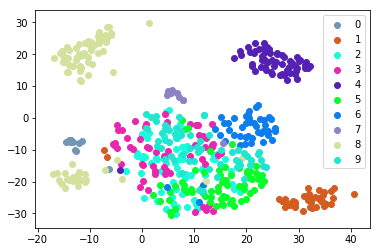
\includegraphics[width=0.35\textwidth]{figs/clusters_CTM}
    \caption{tSNE plot of cells from human melanoma, plotted using Euclidean distances between topic proportions, with cluster assignments shown in color. The cells nicely group into their cluster assignments, suggesting that the clustering topic model inference algorthm worked as intended. Moreover, the cluster assignments correpond to the cell labels found by the group that published the dataset, see Figure \ref{fig:clusters_true} }
    \label{fig:clusters_CTM}
\end{figure}
\begin{figure}
    \centering
    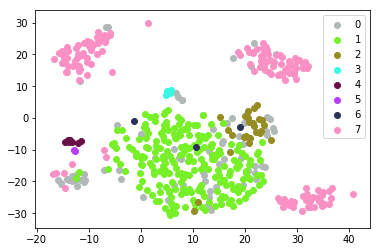
\includegraphics[width=0.35\textwidth]{figs/clusters_true}
    \caption{tSNE plot of cells from human melanoma, plotted using Euclidean distances between topic proportions, with labels published by the group that collected the dataset. 0 - label unknown; 1 - T-cell; 2 - B-cell; 3 - Macrophage; 4 - Endoderm; 5 - Cancer-associated fibroblast; 6 - Natural Killer; 7 - Malignant. The labels correpond to the cluster assignments learned using the CTM model.}
    \label{fig:clusters_true}
\end{figure}

Subsequently, we wanted to determine if the learned topics were meaningful. We first used the biological relevance score described earlier and found that the topics were significantly enriched for some known gene sets from \texttt{MSigDB} (Figure \ref{fig:ctm_pvals}). We then did some examination of the specific genes appearing in select topics using a combination of the \texttt{MSigDB} analysis and \texttt{GO}-enrichment analysis\footnote{\texttt{GO} enrichment analysis looks for enrichment of genes associated with cell processes. Whereas \texttt{MSigDB} is a database of various published gene sets, the \texttt{GO} database contains only those well-characterized gene modules that are generally accepted as being involved in a particular cell process}. We found that topic $18$, which was prevalent in the T-cells and not in other cells (Figure \ref{fig:tcelltopics}), was highly enriched for genes involved in "myeloid dendritic cell activation involved in immune response". Topic $3$, which was prevalent in the B-cells and not elsewhere (Figure \ref{fig:bcelltopics}), was highly enriched for genes involved in "lymphocyte activation" and "inflammatory response". Topic $4$, which was highly prevalent in the T-cells and B-cells only (Figures \ref{fig:tcelltopics} and \ref{fig:bcelltopics}), was highly enriched for genes involved in "somatic diversification of immune receptors". Finally, topic $8$ which was mainly present in the tumor cells (\ref{fig:tumortopics}), was enriched for genes involved in "G1 to S transition of mitotic cell cycle" and "cell division". The correspondence between the genes enriched in the topics and the cell sub-populations with those topics suggests that our learned topics have biological significance. As a result, the highly-ranked genes in some of these topics may be of interest to experimental biologists as candidate gene markers for specific cell sub-populations.

\section{Discussion} 

In this paper, we sought to address the following two questions using Bayesian topic models: given gene expression data, (1) can we identify biologically meaningful gene modules, and (2) can we identify cell sub-populations and find gene modules that illuminate their differences. \\

\subsection{Can we identify biologically meaningful gene modules?}
We addressed the first question by trying to model scRNA-seq data with LDA as well as two non-parametric topic models, the HDP and the IBP-DP. The purpose of doing this was mainly to determine if topic models based on LDA are suitable for modeling gene expression; as far as we are aware, there are no publications applying LDA to scRNA-seq data. Our results from section \ref{ldasec} suggest that LDA could potentially be useful for scRNA-seq, since our topics were enriched for previously discovered biological gene sets. One major consideration is computational cost: although scRNA-seq data is sparse, it is not nearly as sparse as the bag-of-words representation of a corpus, so most inference algorthms take a long time to run on the entire dataset. Based on our results, however, it appears that this problem can be addressed either by using a faster posterior inference method such as online variational inference or by pre-processing the dataset for those genes with the greatest variability.

Compared to LDA, we found that HDP and IBP-DP were not as suitable for modeling scRNA-seq data (Section \ref{nonparametricsec}). The HDP underperformed in comparison to LDA in both log-likelihood on a held-out dataset and the biological significance scores of its topics. The IBP-DP did not seem to work better than LDA on a subset of the Reuters-21578 corpus, based on a qualitative analysis of the topics, so we did not try it on the gene expression data, as we do not expect it to perform better than LDA. The underperformance of the IBP-DP compared to LDA on the Reuters-21578 dataset does not surprise us, as the authors of the IBP-DP paper did not show any topics from their model, even though they claimed it may produce more 'focused' topics.

After we were confident that LDA could be useful for modeling scRNA-seq data, we wanted to try models that could capture higher-level structure of gene expression data - for instance, time. As cells proliferate, they may differentiate into different cell types. A useful topic model might learn not just the topics at a given time point, but also how the topics are evolving over time. We have presented some preliminary results applying a dynamic topic model to our scRNA-seq dataset and selecting an appropriate number of topics (Section \ref{dtmsec}). To further test this model, experiments could be done on simulated time-series scRNA-seq data with known evolving topics, and one could evaluate how well those evolving topics are picked up by the model.

\subsection{Can we identify cell sub-populations and find gene modules that illuminate their differences?}
In addition to time, another source of structure in the scRNA-seq dataset is the clustering of cells into sub-populations. In biology, there is much interest in identifying these sub-populations and finding gene modules or markers that are characteristic of different sub-populations. We first wanted to determine if a Bayesian finite mixture model would be appropriate for separating the cells into clusters (Section \ref{mmsec}). We found that we were approximately able to learn the cell type labels published by \cite{melanoma}\\

Finally, we wanted to create a unified framework for cell clustering and topic modeling. We implemented the clustering topic model (Section \ref{intsec}) and found that it was able to correctly separate the cells into sub-populations. It appeared to outperform the vanilla mixture model without clustering, suggesting that knowledge of the topics helps the model learn better clusters. We also found that several topics corresponded to the cell types that they were prevalent in; we believe these results suggest that biologists can use the topics - which are ranked lists of genes - as candidate gene markers for cell sub-populations of interest within the melanoma, such as malignant cells, T-cells and B-cells. Whether these candidate gene markers are truly useful must be confirmed by biologists experimentally. Looking forward, it would be very interesting to combine the dynamic topic model and the clustering topic model, so that we can capture the time-evolution of the cell sub-populations within a scRNA-seq dataset. 

% In the unusual situation where you want a paper to appear in the
% references without citing it in the main text, use \nocite
% \nocite{langley00}

\section{Author Contributions}
The implementations and experiments involving LDA, Gaussian Mixtures, and the Dynamic Topic Model was completed by SK (Section~\ref{ldasec}, Section~\ref{dtmsec}, and Section~\ref{mmsec}). KY completed the implementations and experiments involved non-parametric topic models, the clustering topic model, and the gene set enrichment test implementation (Section~\ref{nonparametricsec}, Section~\ref{intsec}, and Section~\ref{enrichment_score}). The authors contributed equally in this work.

\bibliography{citations}
\bibliographystyle{sty/icml2013}


\section{Appendix} 

\subsection{Biological Significance Score / Gene Set Enrichment} \label{enrichment_score}
In general, it is difficult to evaluate the 'coherence' of topics of genes, since unlike topics of words, we cannot just read them and get a sense of how similar they are. Therefore, nothing like the intrusion test exists for evaluating topics of genes. To overcome this, we developed our own test for the biological significance of gene topics. The \texttt{MSigDB} contains thousands of gene sets discovered through previous research, catalogued by biologists from the Broad Institute. We deduced that if a topic is 'coherent', then it is likely significantly enriched for some of these gene sets. For each topic, our biological significance scoring method iterates through the \texttt{MSigDB} database and tests each gene set for enrichment using the minimum hyper-geometric test \cite{hg}. The most significant p-values for each topic are recorded and used as a proxy for its biological coherence.

\subsection{Latent Dirichlet Allocation}
\label{ldaappendix}
For our Gibb's sampler, we had a fixed burn-in of number of samples (200), a fixed number of sampling iterations after that (500). We didn't extensively explore varying these values, but trying out significantly more iterations (700) didn't seem to change the topic's word distributions significantly. There was one sampling chain on each of four cores.

\subsection{HDP}
\label{HDP-details}
HDP is an infinite topic extension of LDA based on the Dirichlet process \cite{HDP}. Briefly, words in a corpus are assumed to be generated as follows:
\begin{enumerate}
\item Sample the global distribution over topics, $G_0 \sim$ DP($\gamma, H$), from a Dirichlet process with concentration $\gamma$ and base Dirichlet distribution $H$\footnote{More specifically, $H$ is a Dirichlet distribution over the $(V-1)$-dimensional simplex, where $V$ is the size of the vocabulary, and $G_0$ is a countably infinite set of point masses over this simplex whose weights sum to $1$. $G_0$ in HDP plays a role analogous to $\alpha$ in LDA.}. 
\item For each document $d$,
\begin{enumerate}
\item Sample the local distribution over topics, $G_d \sim$ DP($\alpha_0, G_0$), from a Dirichlet process with concentration $\alpha_0$ and base distribution $G_0$.
\item Choose the number of words in this document, $N_d \sim$ Poisson($\xi$), where $\xi$ is a hyperparameter.
\item For the $i$th word in the $d$th document,
\begin{enumerate}
\item Choose a topic (i.e. distribution over words in vocab), $\beta_{di} \sim$ $G_d$, based on the local distribution over topics
\item Choose a word, $w_{di} \sim$ Categorical($\beta_{di}$), based on the distribution over the vocabulary in the topic
\end{enumerate}
\end{enumerate}
\end{enumerate}

\subsection{IBP-DP}
\label{IBP-details}
One drawback to the HDP is that there tends to be a correlation between how frequently a topic appears across all documents and how prevalent this topic is within documents that it appears in. Williamson et al. \cite{IBP} proposed the 'focused topic model' to overcome this drawback. In their model, the frequency of a topic $k$ depends on two separate variables, its relative prevalence within a document ($\phi_k$) and the probability that a given document contains this topic ($\pi_k$), thus reducing correlation between the two. Briefly, the words in the corpus are assumed to be generated as follows:

\begin{enumerate}
\item For each topic $k = 1, 2, ...$
\begin{enumerate}
\item Choose a population frequency (i.e. probability that a document contains topic) $\pi_k = \prod^k_{j=1} \mu_k$, where each $\mu_k \sim Beta(\alpha, 1)$, where $\alpha$ is a hyperparameter.
\item Choose a relative prevalence (i.e. how often the topic appears within a document containing the topic) $\phi_k \sim Gamma(\gamma, 1)$, where $\gamma$ is a hyperparameter.
\item Choose a distribution over the vocabulary, $\beta_k \sim$ Dir($\eta$), where $\eta$ is a hyperparameter.
\end{enumerate}
\item For each document $d$,
\begin{enumerate}
\item Choose the topics that will appear as a binary vector, $b_d \sim Bernoulli(\pi)$
\item Choose the topic proportion as $\theta_d \sim Dirichlet(b_d\cdot \phi)$
\item Choose the number of words in this document, $N_d \sim$ NegativeBin($\sum_k b_{dk}phi_k$, $\delta$), where $\delta$ is a hyperparameter.
\item For the $i$th word in the $d$th document,
\begin{enumerate}
\item Choose a topic, $z_{di} \sim$ Categorical($\theta_d$), based on the distribution over topics
\item Choose a word, $w_{di} \sim$ Categorical($\beta_{z_{di}}$), based on the distribution over the vocabulary for topic $z_{di}$
\end{enumerate}
\end{enumerate}
\end{enumerate}

\begin{figure*}
    \centering
    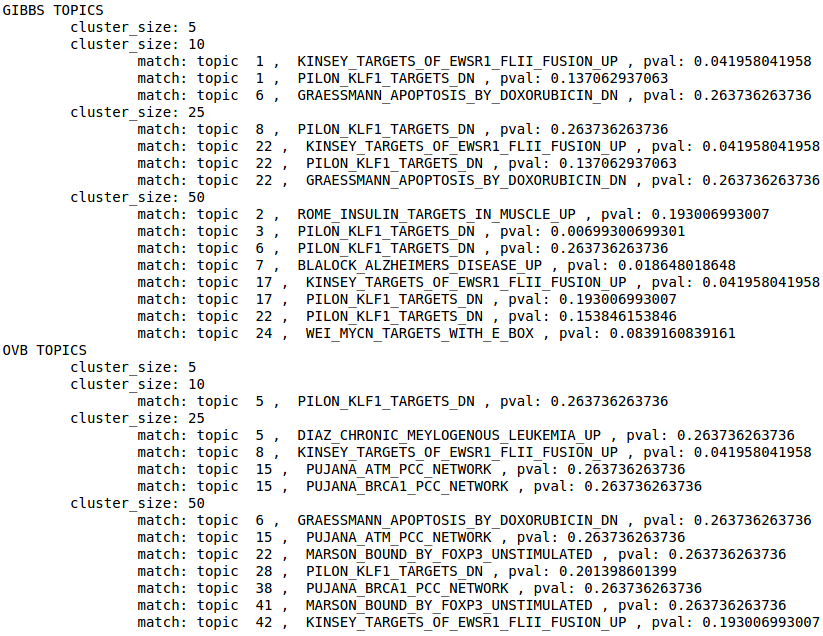
\includegraphics[width=1\textwidth]{figs/pathways}
    \caption{Matches between the gene collections found in LDA topics and published gene sets in \texttt{MSigDB}. `Cluster size' refers to the number of topics in the model}
    \label{fig:pathways}
\end{figure*}

\subsection{Dynamic Topic Model}
\label{dtmappendix}
Here is a description of the generative process for our dynamic topic model:
\begin{enumerate}
    \item Draw a new topic composition hyperparameter \\ $\beta \leftarrow \mathbb{N}(\beta_{t-1}, \sigma I^2)$
    \item Draw a new document composition hyperparameter \\ $\alpha \leftarrow \mathbb{N}(\alpha_{t-1}, \delta I^2)$
    \item For each document: 
    \begin{enumerate}
        \item Draw a new document topic distribution \\ $\theta \leftarrow \pi(\mathbb{N}(\alpha_t))$
        \item For every word in the document:
        \begin{enumerate}
            \item Draw the word topic assignment \\ $Z \leftarrow$ Mult$(\theta)$
            \item Draw the word identity \\ $Z \leftarrow$ Mult$(\pi(\beta_{t,z}))$
        \end{enumerate}
    \end{enumerate}
\end{enumerate}
Here, $\pi(x_i)$ is the softmax function $\frac{exp(x_i)}{\sum_k exp(x_k)}$ \cite{dtm}.

\begin{figure*}
    \centering
    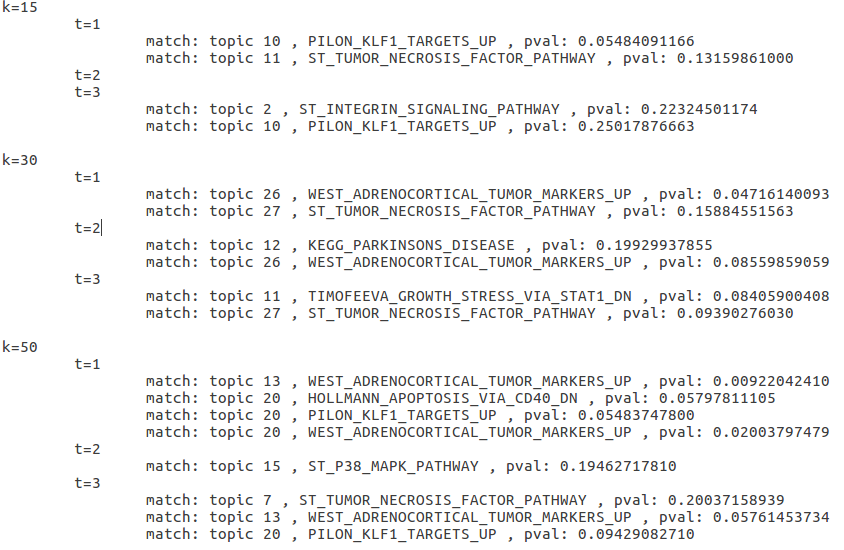
\includegraphics[width=1\textwidth]{figs/pathwaysdtm}
    \caption{Matches between the gene collections found in DTM topics and published gene sets in \texttt{MSigDB}. $k$ refers to the number of topics in the model, $t$ refers to one of three time slices.}
    \label{fig:pathwaysdtm}
\end{figure*}

\begin{figure*}
    \centering
    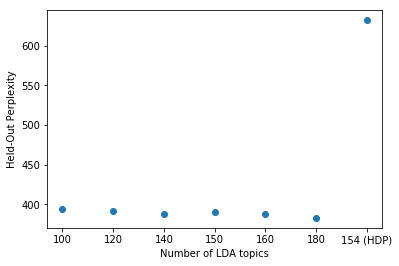
\includegraphics[width=0.5\textwidth]{figs/hdp-perplexity}
    \caption{Comparison of log-likelihood of the held-out testing set, under various LDA models and the HDP model.}
    \label{fig:hdp-perplexity}
\end{figure*}

\begin{figure*}
    \centering
    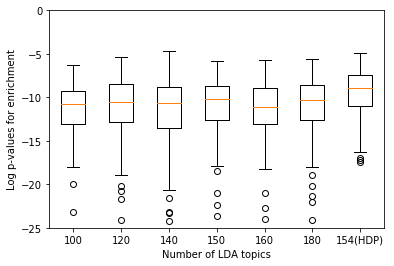
\includegraphics[width=0.5\textwidth]{figs/hdp-enrichment}
    \caption{Comparison of distributions of p-values from gene set enrichment analysis between LDA models and the HDP model.}
    \label{fig:hdp-enrichment}
\end{figure*}

\begin{figure*}
    \centering
    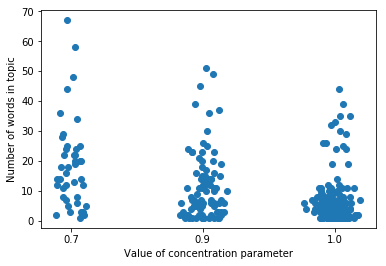
\includegraphics[width=0.5\textwidth]{figs/ibp_words_in_topic}
    \caption{Beeswarm plot of number of words per topic, for 3 different IBP-DP models with different concentration parameters. Each point represents one topic from its model}
    \label{fig:ibp_words_in_topic}
\end{figure*}

\begin{figure*}
    \centering
    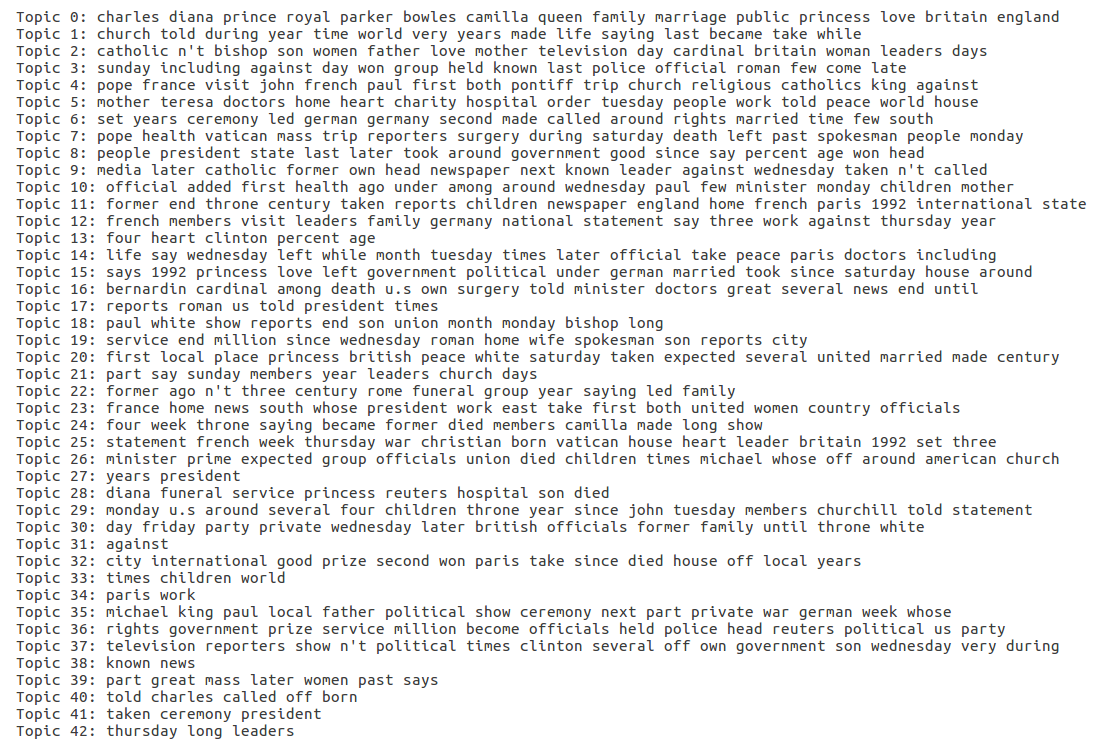
\includegraphics[width=1\textwidth]{figs/ibptopics}
    \caption{Topics from IBP-DP model trained on subset of Reuters dataset.}
    \label{fig:ibptopics}
\end{figure*}

\begin{figure*}
    \centering
    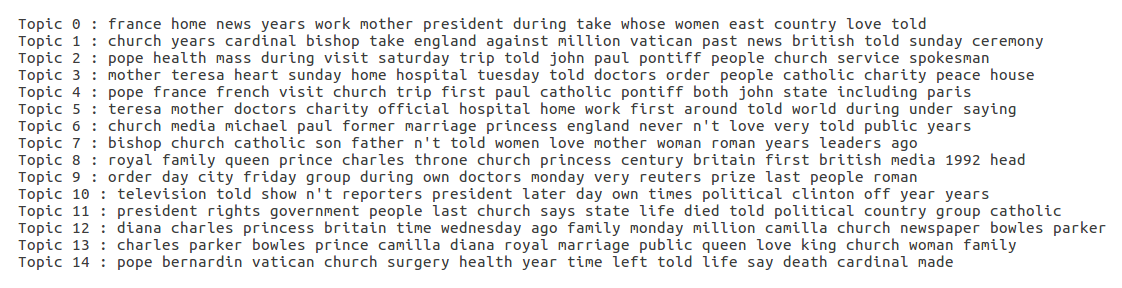
\includegraphics[width=1\textwidth]{figs/ldatopics}
    \caption{Topics from LDA model with 15 topics trained on subset of Reuters dataset.}
    \label{fig:ldatopics}
\end{figure*}

\begin{figure*}
    \centering
    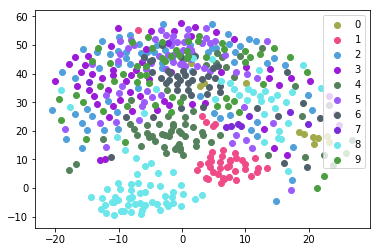
\includegraphics[width=0.35\textwidth]{figs/unclustered}
    \caption{tSNE plot of cells from human melanoma, plotted using Euclidean distances between gene count vectors, with cluster assignments shown in color.}
    \label{fig:unclustered}
\end{figure*}

\begin{figure*}
    \centering
    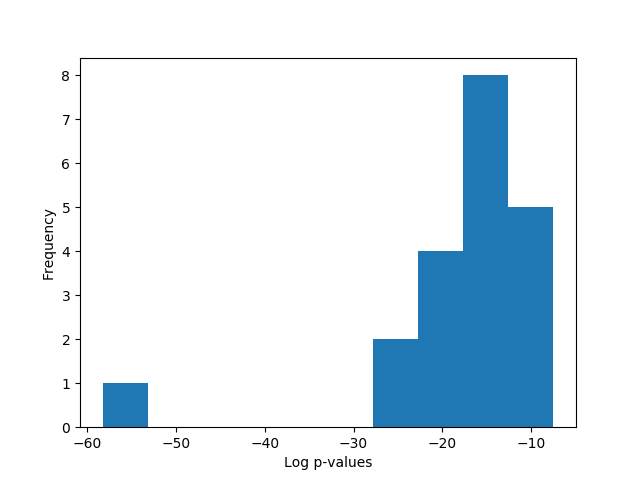
\includegraphics[width=0.35\textwidth]{figs/ctm_pvals}
    \caption{Histogram of topics from CTM model based on p-value of enrichment of \texttt{MSigDB} gene sets.}
    \label{fig:ctm_pvals}
\end{figure*}

\begin{figure*}
    \centering
    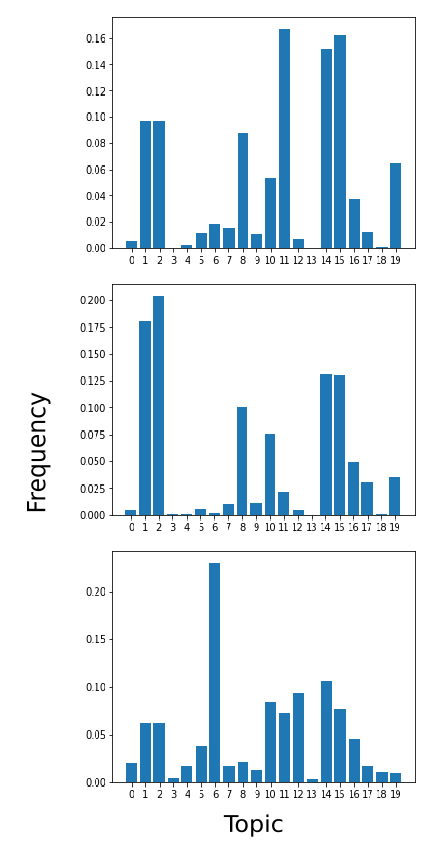
\includegraphics[width=0.35\textwidth]{figs/tumortopics}
    \caption{Bar charts of topic proportions for malignant cell clusters.}
    \label{fig:tumortopics}
\end{figure*}
\begin{figure*}
    \centering
    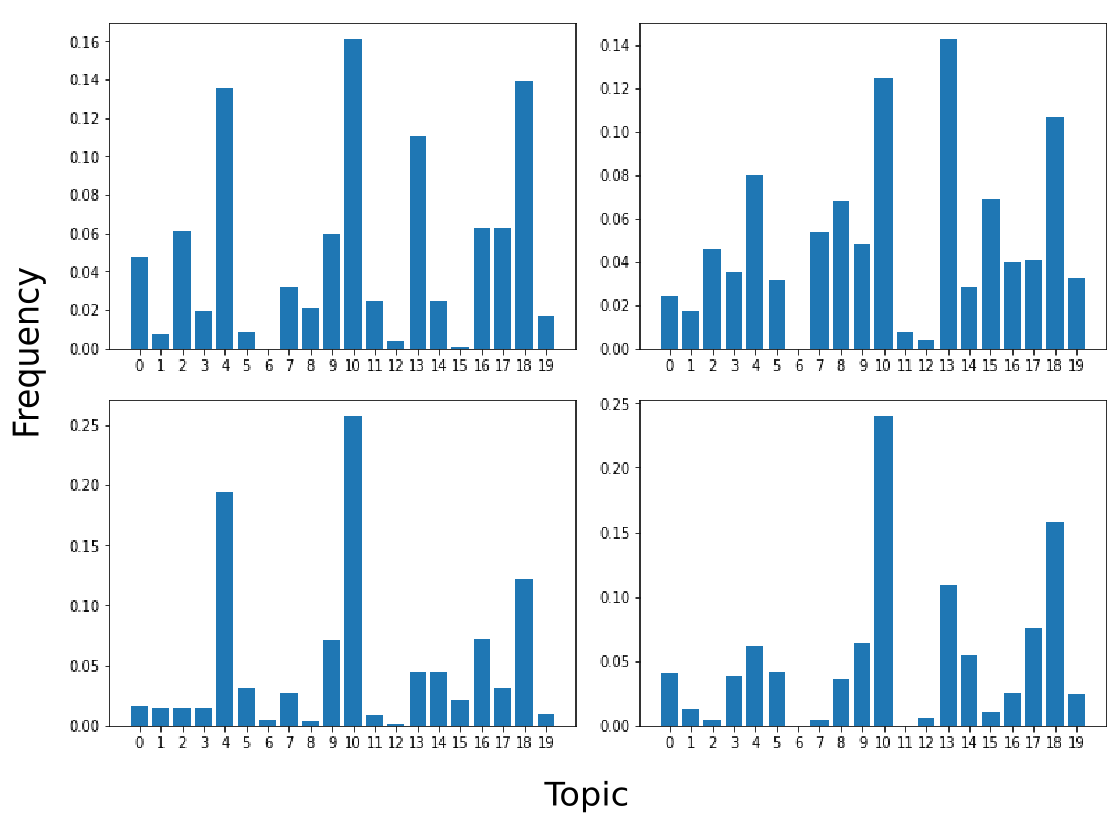
\includegraphics[width=0.5\textwidth]{figs/tcelltopics}
    \caption{Bar charts of topic proportions for T-cell clusters.}
    \label{fig:tcelltopics}
\end{figure*}
\begin{figure*}
    \centering
    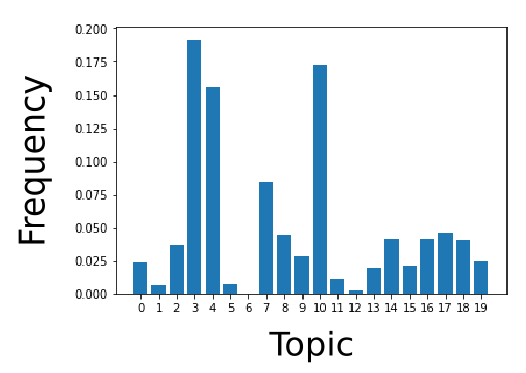
\includegraphics[width=0.35\textwidth]{figs/bcelltopics}
    \caption{Bar charts of topic proportions for B-cell clusters}
    \label{fig:bcelltopics}
\end{figure*}

\end{document} 
